\section{Current Real-Data Evidence}

\paragraph{Registered 100-job study.}
The primary real-data study contains 20 locked seeds on each of BiasBios-Clinical,
Camelyon17-WILDS, CivilComments-WILDS, GaitPDB, and Waterbirds. Each job evaluates
the same 13-candidate family built with the official INLP, LEACE, R-LACE, TaCo,
and MANCE++ implementations. The strict-v2 replay reproduces all 100 decisions;
an exact-rational audit verifies 1,300 bridge certificates and 1,400 release
bounds. Table~\ref{supp:tab:current-real-rules} gives the aggregate comparison
at the primary $.40$ worst-stratum error contract.

\begin{table*}[t]
\centering
\small
\setlength{\tabcolsep}{3.7pt}
\begin{tabular}{lrrr}
\hline
Rule & Released & Estimable & Diagnostic violations \\
\hline
Strict MOSAIC & 20 & 20 & 0 \\
Direct target-table certificate & 36 & 36 & 0 \\
Bridge plug-in & 47 & 47 & 7 \\
Validation-only selection & 80 & 60 & 18 \\
Unconditional selection & 100 & 80 & 38 \\
\hline
\end{tabular}
\caption{Aggregate primary-contract outcomes over 100 registered jobs. The
direct target-table rule certifies the sampled target table; strict MOSAIC
certifies the registered bridge-admitted population class.}
\label{supp:tab:current-real-rules}
\end{table*}

Strict MOSAIC releases 20 BiasBios-Clinical interfaces at every registered
threshold from $.30$ through $.45$, and 23 interfaces at $.49$; every released
job has an estimable untouched diagnostic and no observed diagnostic violation.
The direct target-table comparator releases 36 jobs with no observed diagnostic
violation. Its guarantee applies to the target table itself, whereas MOSAIC's
bridge program certifies a structured class of target laws. The bridge plug-in,
which keeps the learned transform but omits the confidence event, releases 47
jobs and records seven diagnostic violations. This side-by-side comparison
separates target-table certification from transport certification and quantifies
the value of the simultaneous regions.

\begin{figure*}[t]
  \centering
  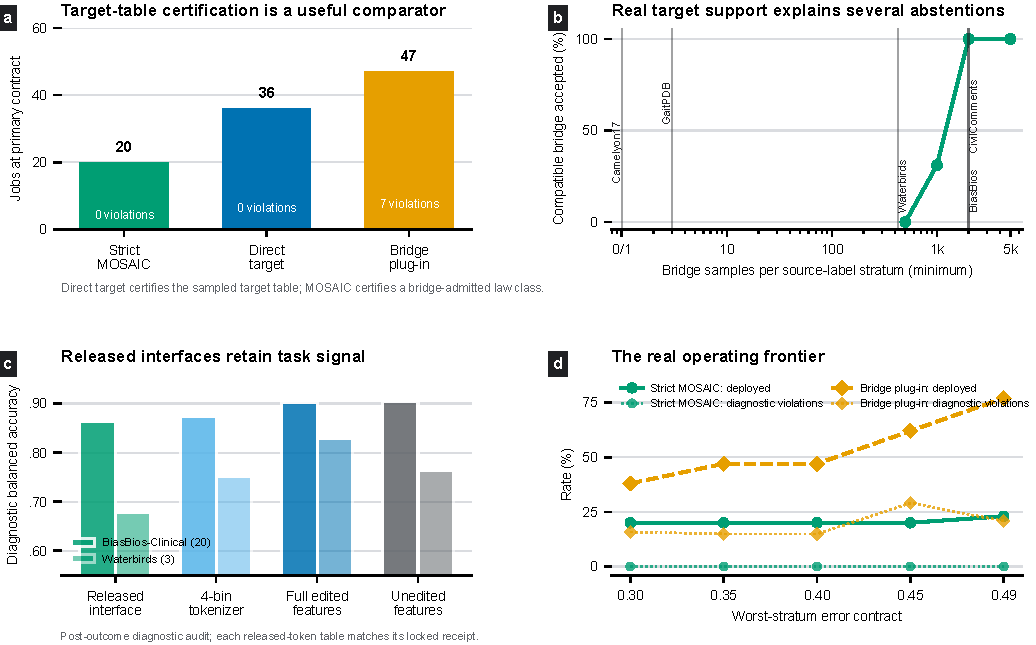
\includegraphics[width=\textwidth]{figures/figure4_mosaic_revision_evidence.pdf}
  \caption{Additional audited evidence. (a) The direct target-table rule
  releases 36/100 jobs; strict MOSAIC releases 20/100 under the
  bridge-admitted population class. (b) Real bridge stratum support is overlaid
  on the locked bridge-power curve. (c) The released interfaces retain task
  signal on untouched diagnostics. (d) Deployment and observed
  diagnostic-violation rates across the registered utility frontier.}
  \label{supp:fig:current-real-evidence}
\end{figure*}

\paragraph{California-to-Texas confirmation.}
Five fresh ACSIncome jobs use California as the reference population and Texas
as the labeled target population. The task is income above \$50,000; binary sex
is the audit source and is excluded from released features. Five locked seeds
evaluate the complete official 13-candidate frontier. The independent strict
replay checks all 65 candidate rows and 70 global optimizations. At the $.40$
primary contract, MOSAIC abstains on all five jobs. At the registered $.45$
and $.49$ contracts, it releases all five jobs: three R-LACE and two identity
interfaces. Every released interface satisfies its untouched Texas diagnostic.
